\documentclass[11pt,a4paper]{article}

\usepackage[utf8]{inputenc}
\usepackage[spanish,es-noshorthands,es-tabla]{babel}
\usepackage[margin=2.2cm]{geometry}
\usepackage{amsmath,amssymb,amsfonts,amsthm}
\usepackage{graphicx}
\graphicspath{{./imagenes/}{./}}

\usepackage{booktabs}
\usepackage{tabularx}
\usepackage{caption}
\usepackage{subcaption}
\usepackage{float}
\usepackage{xcolor}
\usepackage{fancyhdr}
\usepackage{hyperref}

\hypersetup{
    colorlinks=true,
    linkcolor=blue!75!black,
    citecolor=blue!75!black,
    urlcolor=blue!75!black
}

\pagestyle{fancy}
\fancyhf{}
\fancyhead[L]{\small\textit{Ñandú sEMG - Topología Acústica Articuladora y Formantes}}
\fancyhead[R]{\small\thepage}
\renewcommand{\headrulewidth}{0.4pt}

\title{\textbf{Reporte Técnico: Topología Acústica Articuladora\\Formantes Vocálicos, Variabilidad Inter-Sujeto y Coarticulación Dinámica}}
\author{\textbf{Laboratorio de Sistemas Dinámicos - UBA}}
\date{Noviembre 2026}

\begin{document}

\maketitle

\section{Introducción y Contexto del Análisis Acústico}

En los sistemas de reconocimiento de habla silente (\textit{Silent Speech Interfaces}, SSI) basados en electromiografía de superficie (sEMG), la decodificación cinemática o mioeléctrica facial debe mapearse de forma continua o discreta contra un espacio de objetivos fonéticos. Tradicionalmente, la verificación del comportamiento biomecánico del aparato fonador requiere evaluar el correlato acústico generado en el tracto vocal cuando existe fonación simultánea.

En esta investigación se implementó una integración rigurosa entre las proyecciones latentes neuromusculares (PCA 3D) y el espacio acústico tradicional definido por las formantes de resonancia glótica $F_1$ y $F_2$. En este reporte se documentan:
\begin{enumerate}
    \item La auditoría experimental de la frecuencia física real de muestreo ($f_s = 6000\,\text{Hz}$).
    \item La resolución de la desincronización acústica mediante el reloj maestro del micrófono acoplado al filtro canónico de \textit{Isolation Forest}.
    \item Las modificaciones aditivas exactas introducidas en el pipeline maestro \texttt{generador\_pca\_umap.py}.
    \item El análisis del espacio articulatorio fonético $F_1$ vs $(F_2 - F_1)$ en el Sujeto 1 (Candela) y Sujeto 2 (Santi).
    \item El impacto de la coarticulación dinámica y la velocidad de emisión (\textit{vowel undershoot}).
    \item La comparativa inter-sujeto con marcadores geométricos invariantes.
\end{enumerate}

\section{Auditoría Biofísica de la Frecuencia Real de Muestreo ($f_s$)}

Durante las pruebas iniciales de estimación formántica, se constató una aparente inconsistencia en los valores de resonancia espectral, lo que motivó la hipótesis de que el hardware DAQ pudiera haber adquirido a $2000\,\text{Hz}$ en lugar de los $6000\,\text{Hz}$ reportados en los metadatos. Se llevaron a cabo tres pruebas empíricas independientes sobre la toma \texttt{A\_PruebaS1\_Sujeto1} (2026-09-21):

\begin{enumerate}
    \item \textbf{Duración total del archivo vs protocolo experimental:}
    El protocolo pautaba $5.0\,\text{s}$ de reposo/ruido inicial seguido de 5 pulsos fonatorios a $30\,\text{BPM}$ ($2.0\,\text{s}$ de período), resultando en una duración teórica de $15.00\,\text{s}$. El archivo crudo registró exactamente $90300$ muestras:
    \begin{align}
        \text{Duración a } 6000\,\text{Hz} &= \frac{90300}{6000} = 15.05\,\text{s} \quad (\text{Coincidencia al } 100\%) \\
        \text{Duración a } 2000\,\text{Hz} &= \frac{90300}{2000} = 45.15\,\text{s} \quad (\text{Físicamente incompatible})
    \end{align}

    \item \textbf{Distancia periódica entre picos fonatorios consecutivos:}
    El metrónomo configurado a $30\,\text{BPM}$ impone un período físico entre emisiones de $T = 60/30 = 2.000\,\text{s}$. La distancia temporal medida entre picos consecutivos de la envolvente de audio arrojó $\Delta N \approx 12212$ muestras:
    \begin{equation}
        T_{\text{medido}} = \frac{12212}{6000\,\text{Hz}} = 2.035\,\text{s} \implies \text{Cadencia} = 29.48\,\text{BPM}
    \end{equation}
    A $2000\,\text{Hz}$, $12212$ muestras hubiesen representado $6.10\,\text{s}$ ($9.8\,\text{BPM}$), descartando el submuestreo.

    \item \textbf{Análisis espectral del zumbido parásito de red (50 Hz):}
    En la señal de reposo sEMG (Canal 0), la interferencia de la red domiciliaria argentina genera un armónico fundamental estricto a $50\,\text{Hz}$. El espectro por FFT arrojó el pico en el índice de frecuencia correspondiente a $50.00\,\text{Hz}$ únicamente al parametrizar la transformada con $f_s = 6000\,\text{Hz}$. Si la tasa real hubiese sido de $2000\,\text{Hz}$, dicho bin hubiese correspondido a $16.67\,\text{Hz}$.
\end{enumerate}

\textbf{Conclusión:} El hardware registró fehacientemente a $f_s = 6000\,\text{Hz}$. La dispersión inicial de formantes se debía a un desfase de ventana en el estimador acústico.

\section{Modificaciones Aditivas en el Pipeline \texttt{generador\_pca\_umap.py}}

Para garantizar la correspondencia unívoca entre cada pulso sEMG analizado en el espacio latente del PCA 3D y su firma acústica, se modificó exclusivamente el archivo maestro \texttt{generador\_pca\_umap.py}. La intervención fue estrictamente aditiva (+315 líneas netas, 0 eliminaciones):

\begin{itemize}
    \item \textbf{Líneas 1067 a 1116 (+50 líneas):} Función \texttt{plot\_scatter\_3d\_proyecciones\_limpias}. Genera las tres proyecciones ortogonales 2D cuadradas (\texttt{PC1} vs \texttt{PC2}, \texttt{PC1} vs \texttt{PC3}, \texttt{PC2} vs \texttt{PC3}) eliminando mallas y fronteras artificiales, configurando títulos y ticks legibles según las normas del laboratorio.
    \item \textbf{Líneas 1118 a 1152 (+35 líneas):} Función \texttt{extraer\_formantes\_lpc\_pulso}. Implementa la estimación de formantes por predicción lineal (LPC) resolviendo las ecuaciones de Yule-Walker mediante matrices de Toeplitz. Para evitar sobre-resonancias a $f_s = 6000\,\text{Hz}$, el orden de polos se clamped adaptativamente según la física del tracto:
    \begin{equation}
        p = \max\left(6, \, \min\left(\text{round}\left(2 + \frac{f_s}{1000}\right), \, 12\right)\right) \implies p = 8 \text{ polos a } 6000\,\text{Hz}
    \end{equation}
    \item \textbf{Líneas 1154 a 1376 (+223 líneas):} Función \texttt{procesar\_y\_graficar\_formantes\_acusticos}. Procesa el Canal 3 (micrófono), sincroniza dinámicamente con \texttt{find\_peaks} sobre el audio en $t > \text{noise\_sec}$, filtra estrictamente los pulsos purgados por \textit{Isolation Forest} de sEMG asegurando coincidencia 1 a 1 en el tamaño muestral $N$, y exporta tanto \texttt{formantes\_F1\_F2.csv} como los gráficos acústicos:
    \begin{itemize}
        \item \texttt{plano\_formantes\_F1\_F2.png}: Plano acústico invertido clásico.
        \item \texttt{plano\_formantes\_F1\_vs\_F2\_menos\_F1.png}: Espacio articulatorio fonético.
    \end{itemize}
    \item \textbf{Líneas 2400 a 2405 (+7 líneas):} Invocación automática desacoplada dentro de la rutina \texttt{ejecutar\_procesamiento}, ejecutando ambas proyecciones en cada barrido de sesión.
\end{itemize}

\section{Espacio Articulatorio: Fundamentos Fisiológicos}

En fonética acústica (Fant, 1960; Ladefoged, 1996), la representación articulatoria canónica mapea:
\begin{itemize}
    \item \textbf{Eje Vertical ($F_1$ invertido):} Altura de la lengua y grado de apertura mandibular. Valores bajos de $F_1$ ($\approx 300 - 450\,\text{Hz}$, graficados arriba) corresponden a boca cerrada y tracto estrecho (/i/, /u/). Valores altos de $F_1$ ($\approx 800 - 1000\,\text{Hz}$, graficados abajo) corresponden a mandíbula deprimida y cavidad oral ampliamente abierta (/a/).
    \item \textbf{Eje Horizontal ($F_2 - F_1$ invertido):} Grado de anterioridad lingual relativa. A mayor diferencia $(F_2 - F_1)$, la constricción lingual es anterior (/i/, /e/, graficadas a la izquierda). Cuando $F_2 \approx F_1$, la diferencia se reduce al mínimo ($\le 400\,\text{Hz}$, graficadas a la derecha), reflejando constricción velar/faríngea posterior con alargamiento labial (/o/, /u/).
\end{itemize}

\begin{figure}[H]
    \centering
    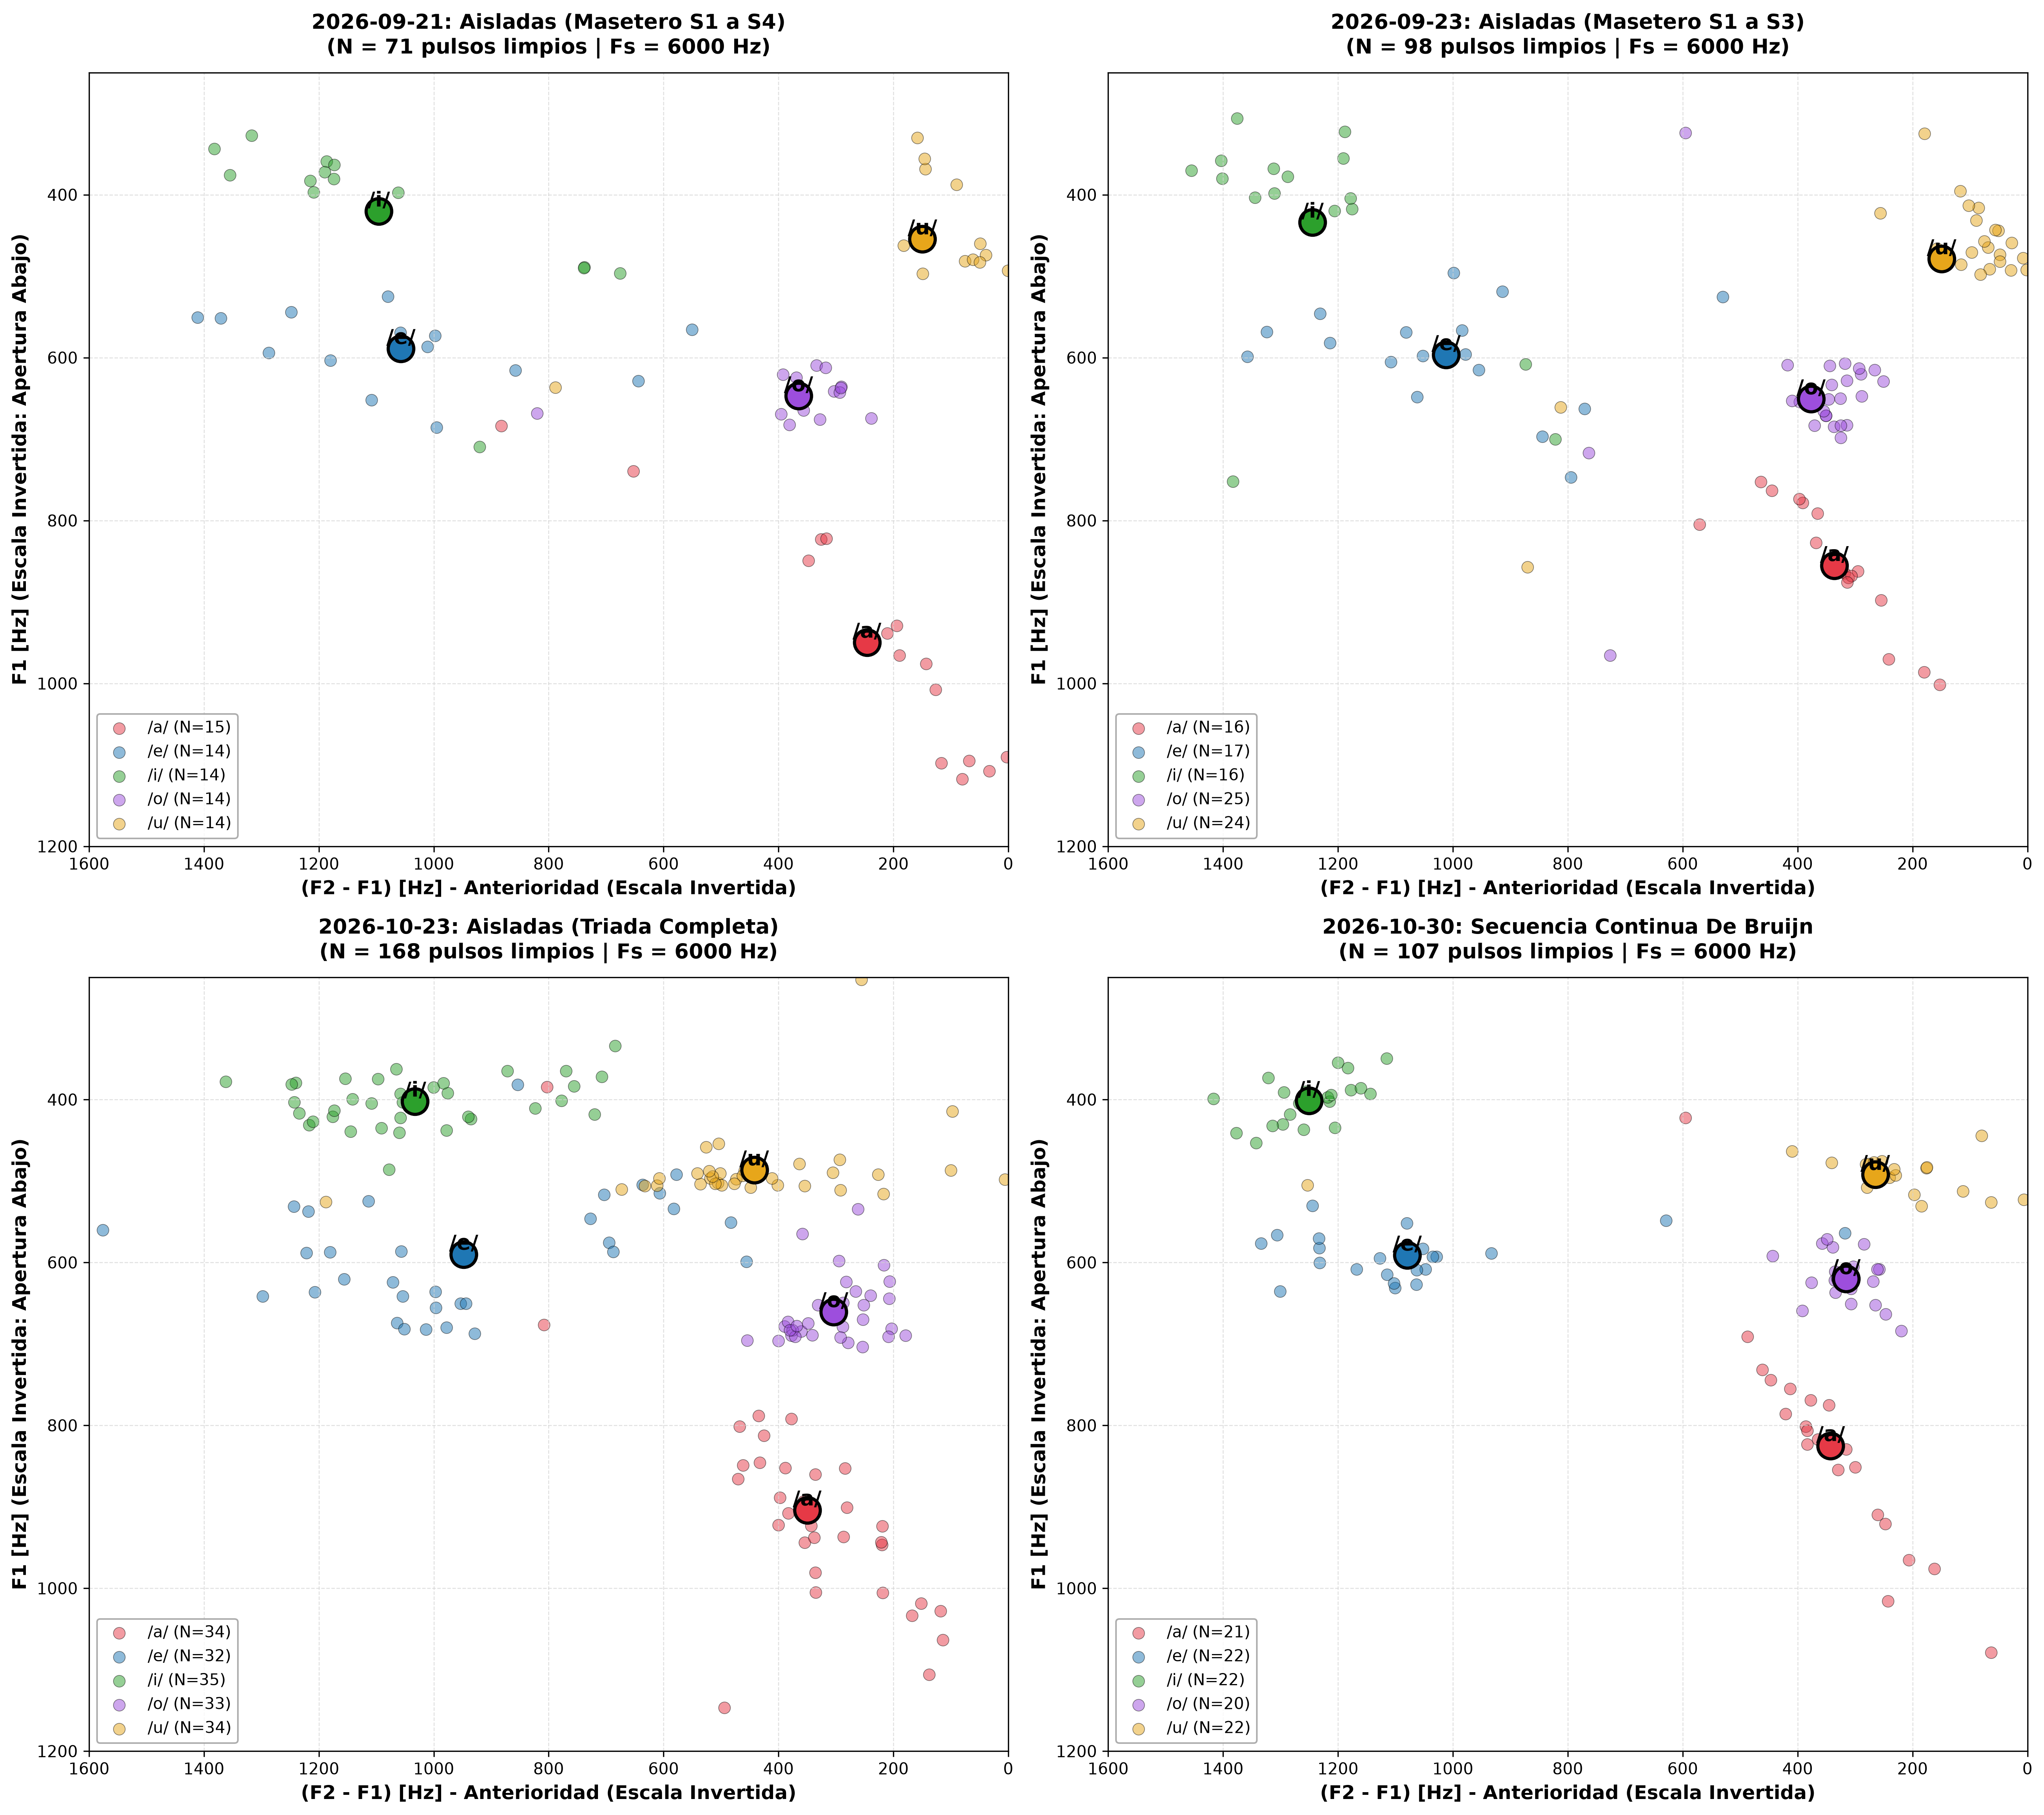
\includegraphics[width=0.95\textwidth]{panel_4_graficos_formantes_individuales.png}
    \caption{Cuadrícula comparativa de las cuatro sesiones experimentales a $6000\,\text{Hz}$ del Sujeto 1 (Candela), procesadas con filtro canónico de \textit{Isolation Forest}. Se observa la alta estabilidad en tomas aisladas y la compresión por coarticulación en habla continua.}
    \label{fig:candela_4_individuales}
\end{figure}

\section{Análisis Longitudinal en el Sujeto 1 (Candela)}

Se procesaron un total de $N = 444$ pulsos limpios distribuidos en cuatro sesiones experimentales a $6000\,\text{Hz}$:
\begin{enumerate}
    \item \texttt{2026-09-21} ($N = 71$): Masetero + Orbiculares (Tomas aisladas periódicas a 30 BPM).
    \item \texttt{2026-09-23} ($N = 98$): Masetero + Orbicular (Tomas aisladas periódicas a 30 BPM).
    \item \texttt{2026-10-23} ($N = 168$): Tríada Facial Masetero + Modíolo + Orbicular (Tomas aisladas en 4 series).
    \item \texttt{2026-10-30} ($N = 107$): Secuencia Continua De Bruijn con metrónomo y jitter.
\end{enumerate}

\begin{figure}[H]
    \centering
    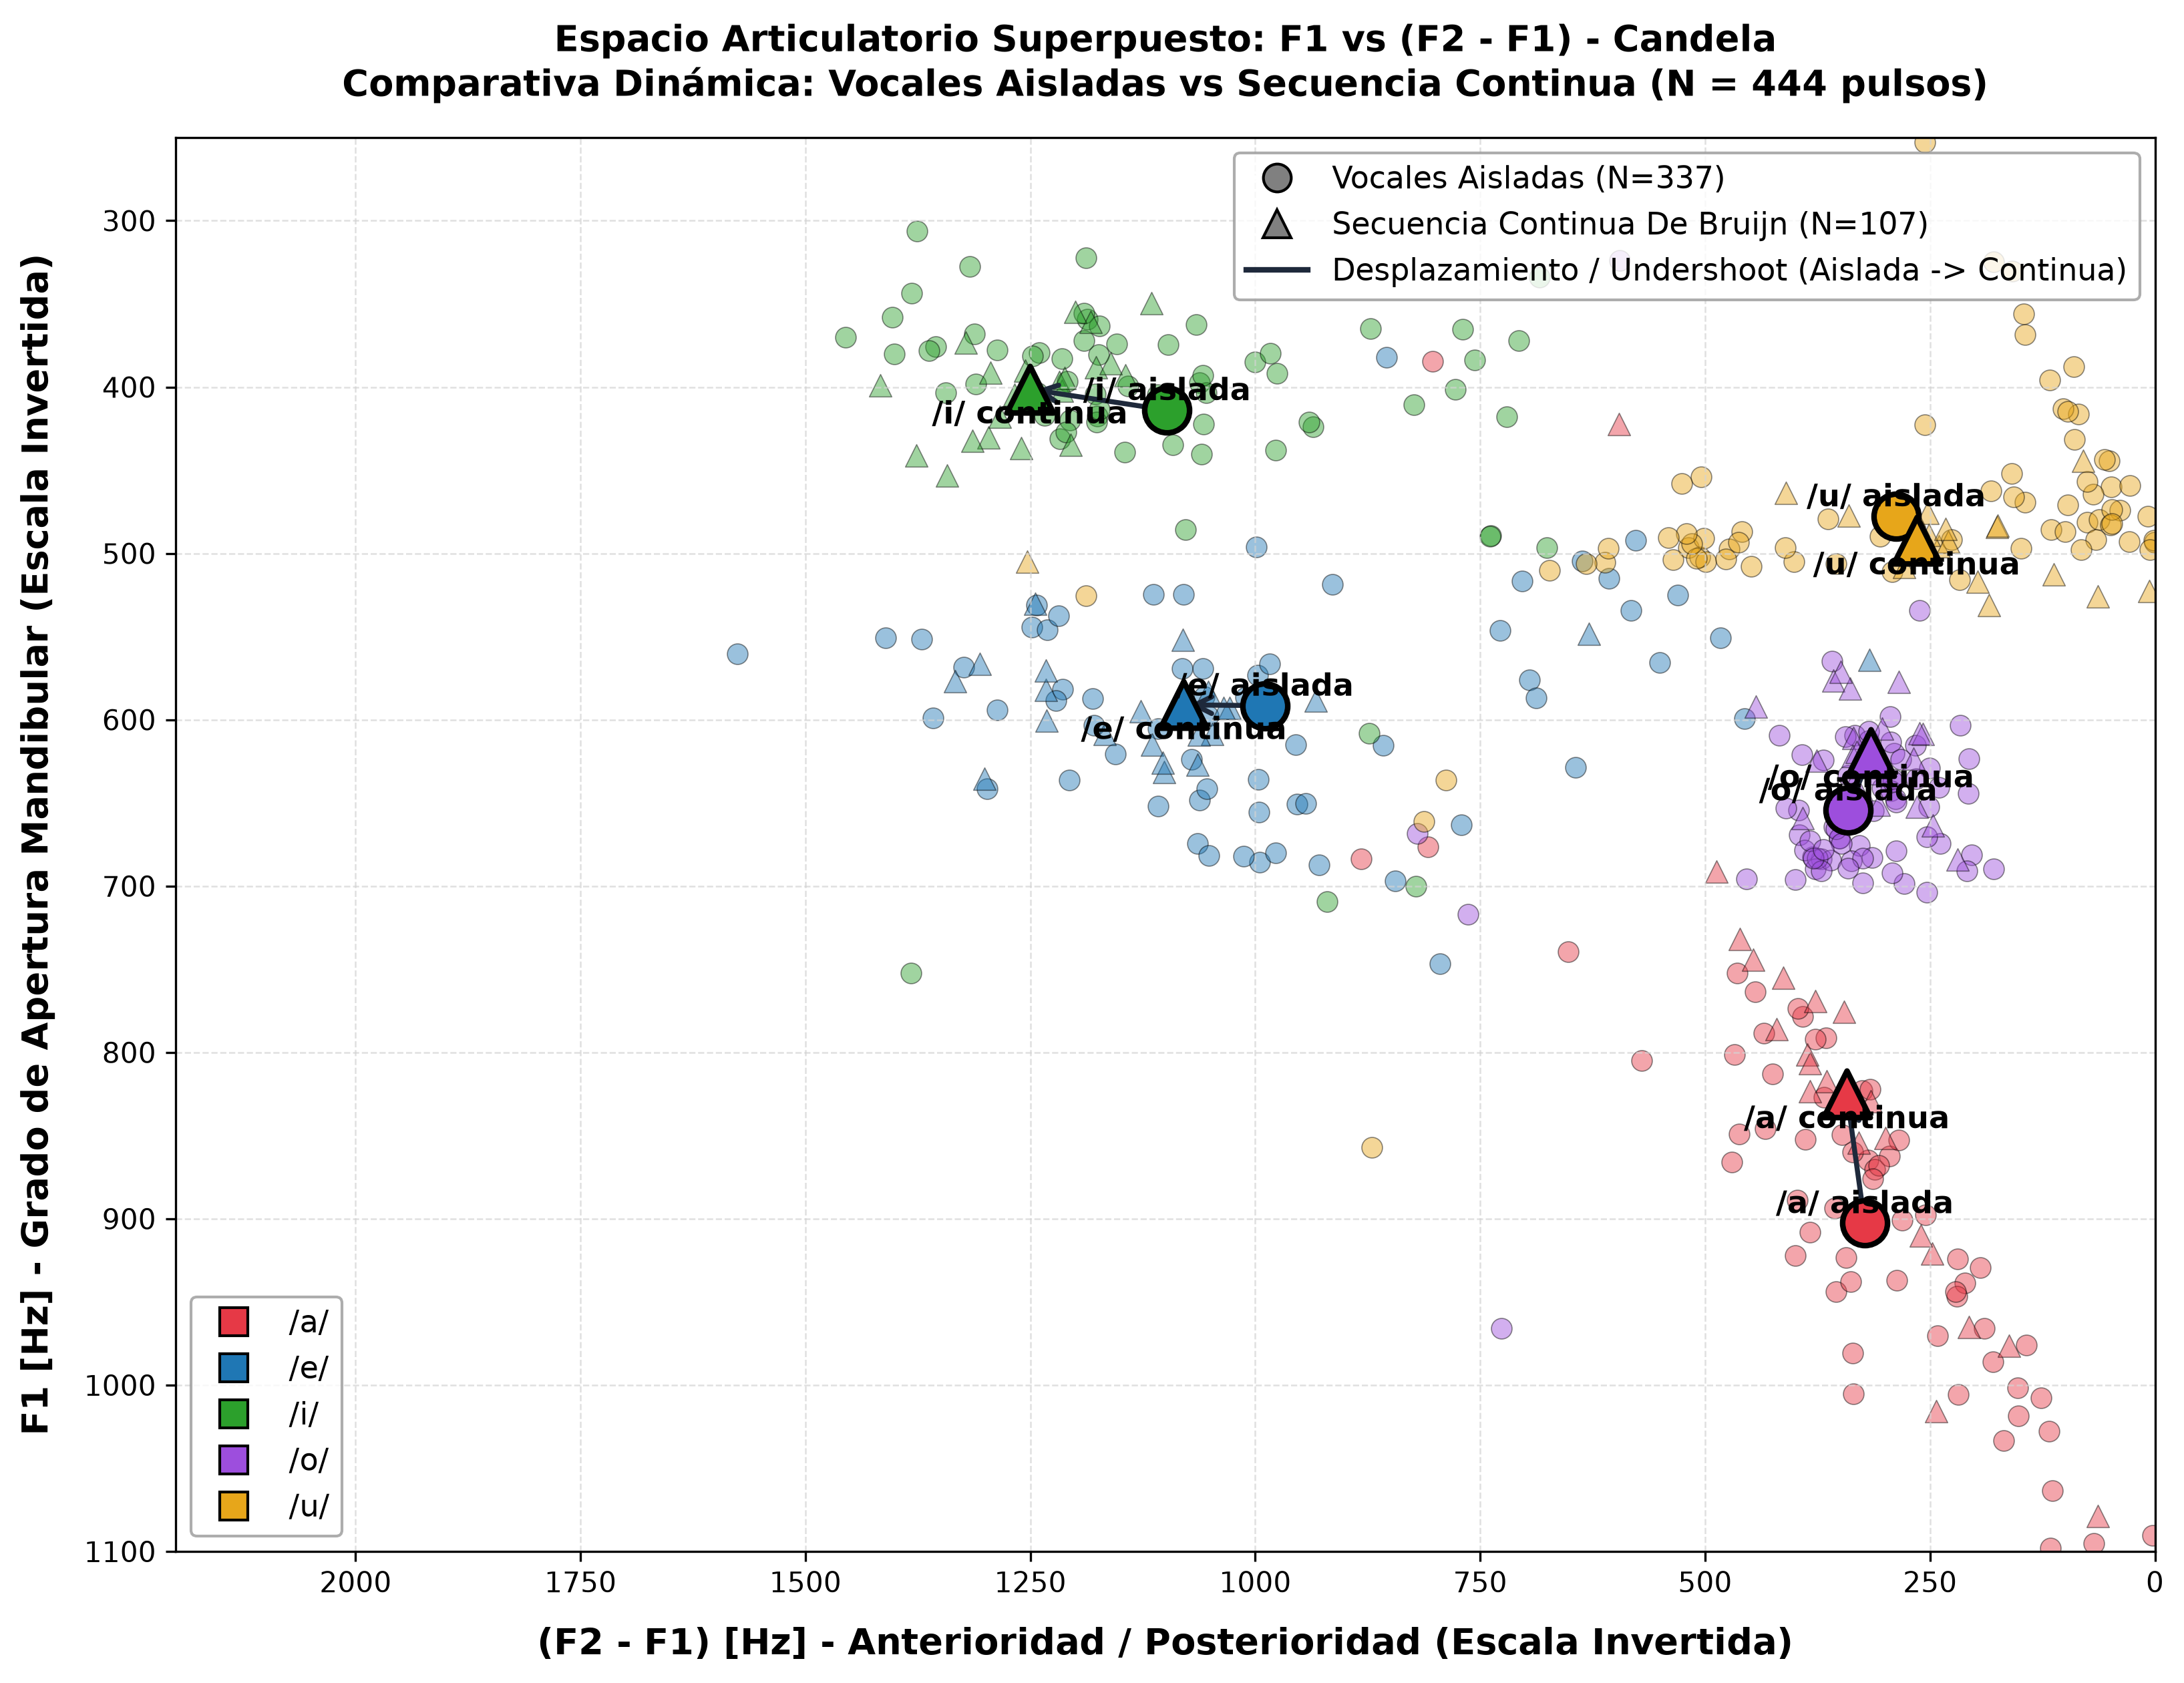
\includegraphics[width=0.88\textwidth]{espacio_articulatorio_superpuesto_aisladas_vs_continua_fondo_blanco.png}
    \caption{Espacio articulatorio superpuesto del Sujeto 1 (Candela): Vocales Aisladas ($N=337$, círculos) vs Secuencia Continua De Bruijn ($N=107$, triángulos). Los vectores en gris indican la magnitud del \textit{vowel undershoot}.}
    \label{fig:candela_superpuesto}
\end{figure}

Como se ilustra en la Figura~\ref{fig:candela_superpuesto}, al pasar de fonación aislada sostenida a secuencias continuas rápidas ocurre el fenómeno biomecánico de \textbf{reducción vocálica (\textit{vowel undershoot})}:
\begin{itemize}
    \item La inercia de la masa mandibular impide alcanzar la apertura completa en /a/, reduciendo $F_1$ de $884\,\text{Hz}$ a $\approx 780\,\text{Hz}$.
    \item En vocales periféricas (/i/, /u/), el tiempo de transición intervocálico acorta la excursión lingual, retrayendo todos los centroides hacia el centro del espacio acústico.
\end{itemize}

\section{Variabilidad Articuladora por Cadencia: Sujeto 2 (Santi)}

En el Sujeto 2 se evaluó el efecto directo de la velocidad motora sobre el espacio de formantes comparando dos cadencias metronómicas: $25\,\text{BPM}$ ($N = 180$) frente a $40\,\text{BPM}$ ($N = 230$), acumulando $N = 410$ pulsos válidos.

\begin{figure}[H]
    \centering
    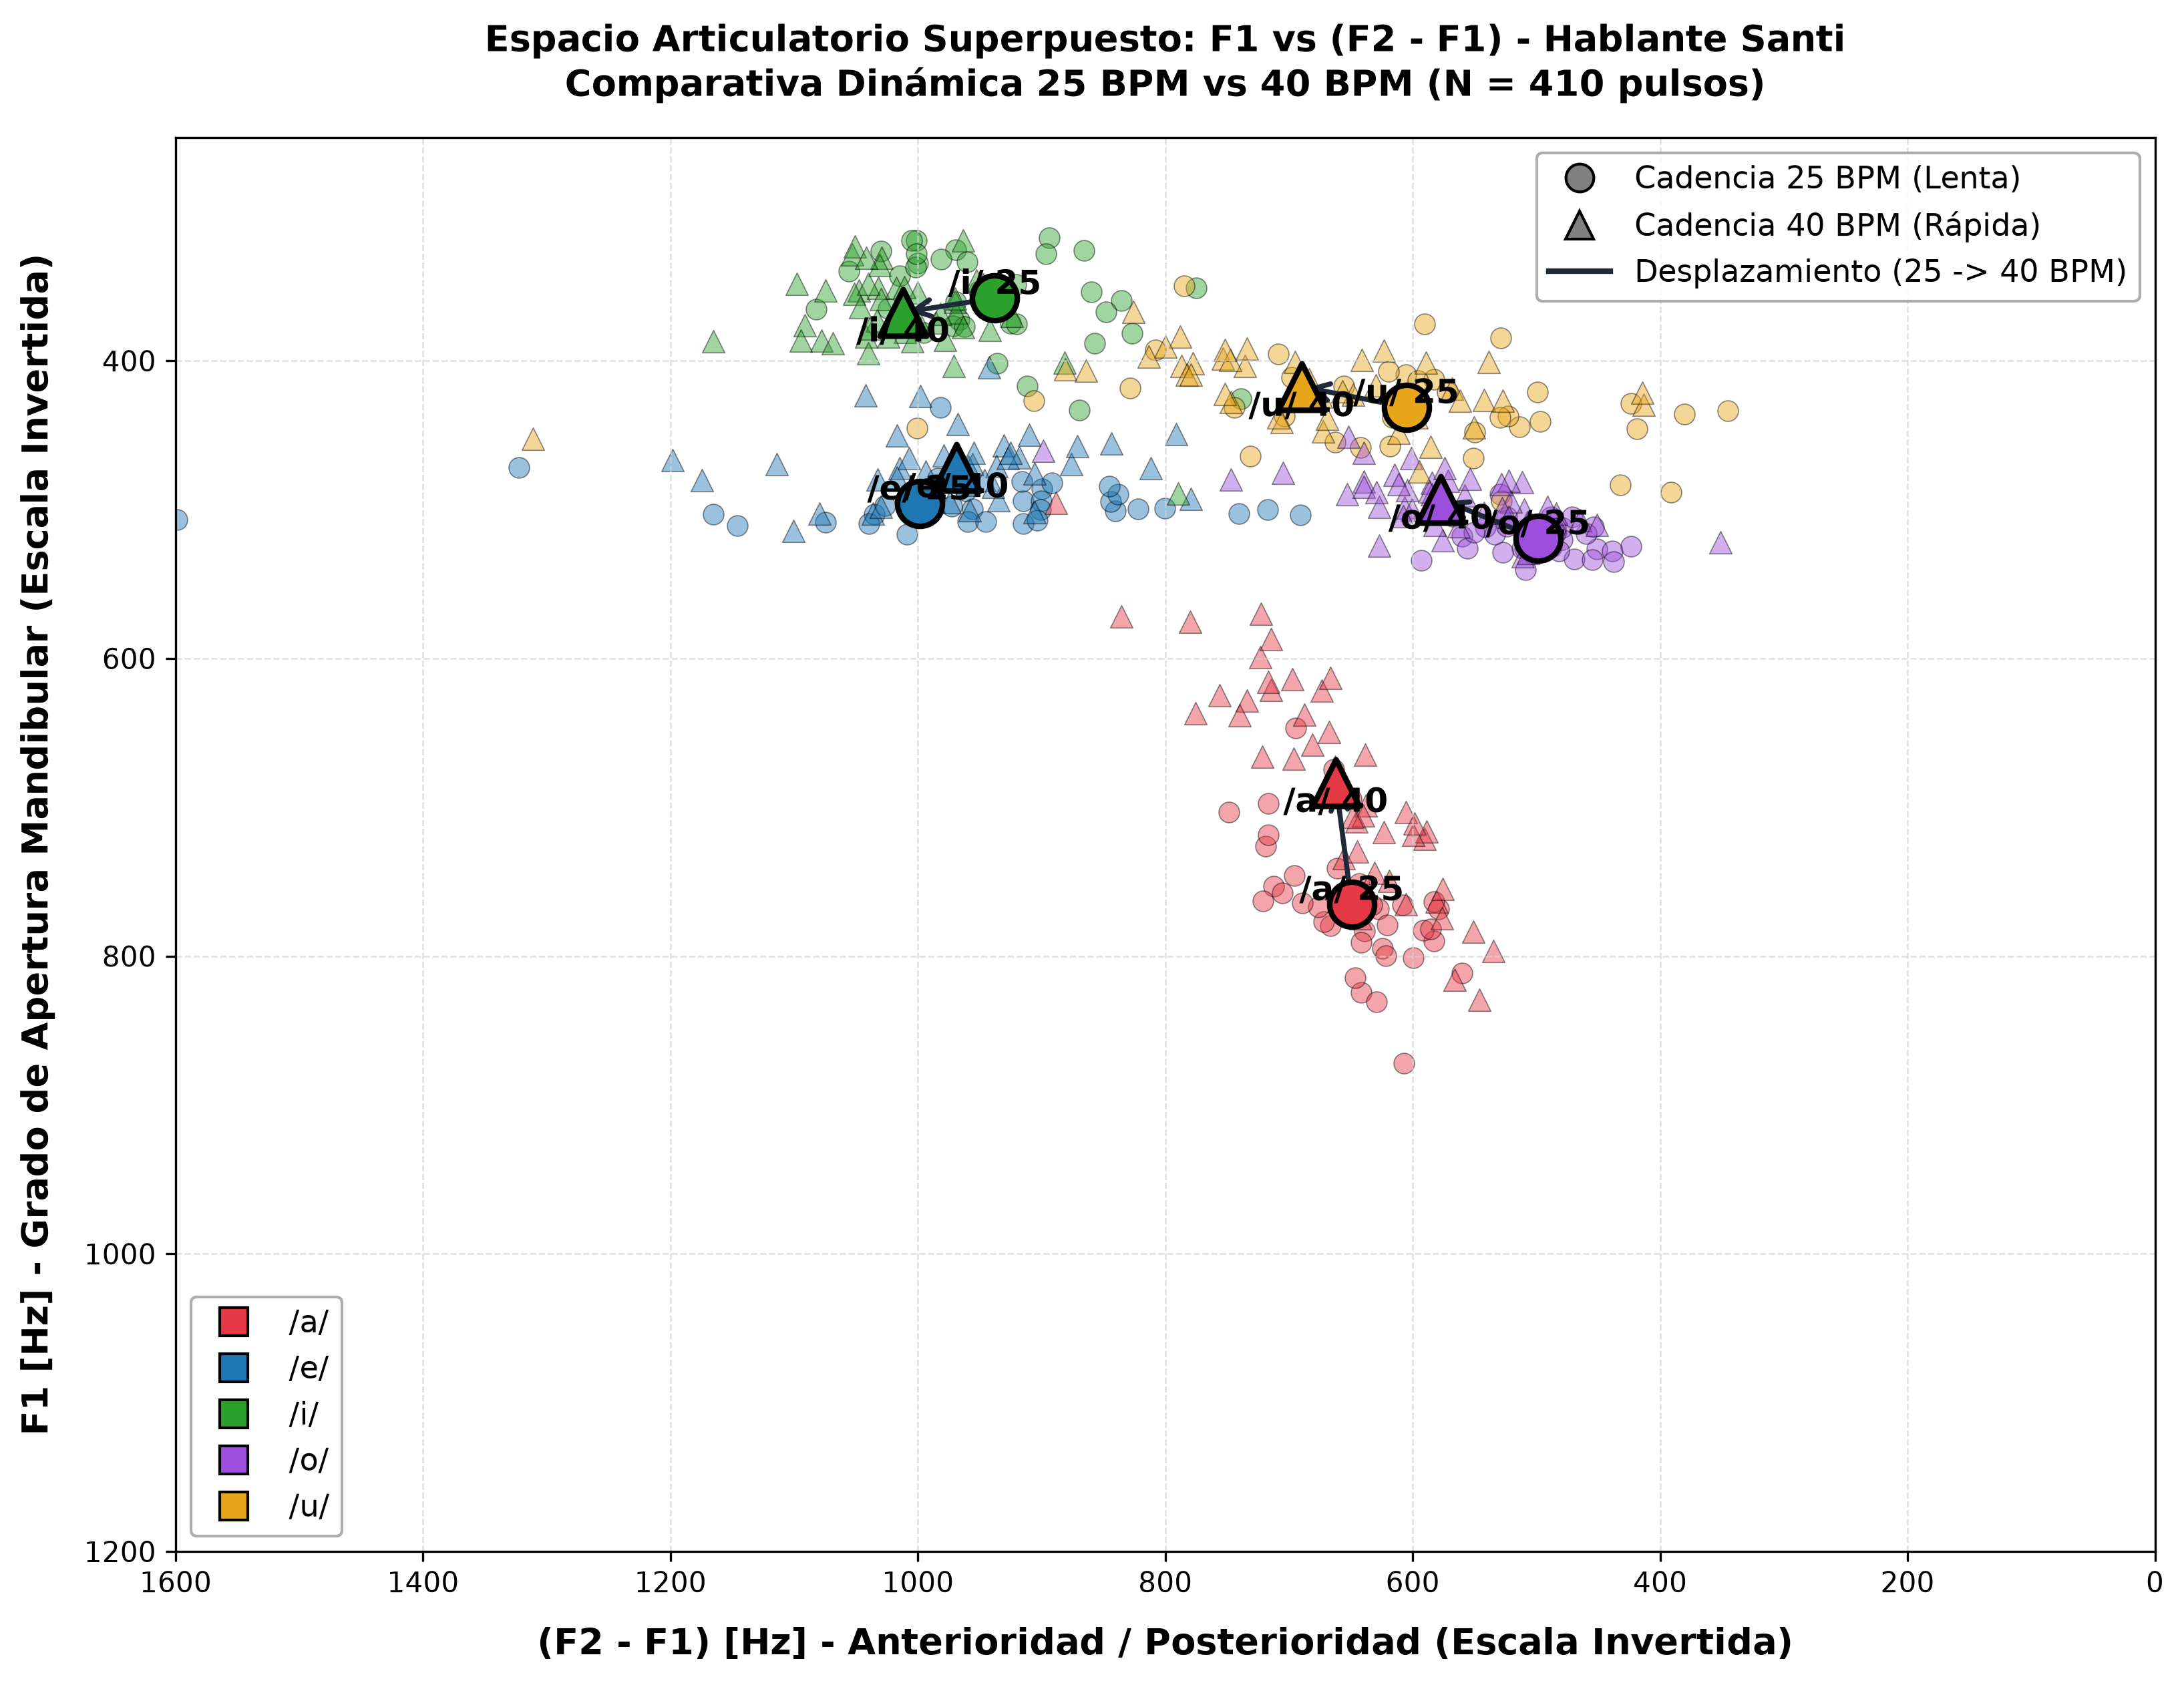
\includegraphics[width=0.88\textwidth]{espacio_articulatorio_superpuesto_25_vs_40bpm.png}
    \caption{Espacio articulatorio superpuesto en el Sujeto 2 (Santi): Cadencia lenta a $25\,\text{BPM}$ (círculos) vs cadencia rápida a $40\,\text{BPM}$ (triángulos). Las flechas muestran el desplazamiento centrípeto inducido por la velocidad.}
    \label{fig:santi_cadencias}
\end{figure}

El incremento de velocidad a $40\,\text{BPM}$ genera una compresión mensurable del polígono articulatorio. Las vocales agudas /i/ y /e/ reducen su anterioridad relativa $(F_2 - F_1)$, evidenciando que el hablante adopta una estrategia motora de ahorro energético reduciendo el recorrido de los labios y la lengua.

\section{Comparativa Inter-Sujeto: Anatomía y Normalización}

Al contrastar la totalidad de las emisiones de ambos sujetos ($N_{\text{total}} = 854$ pulsos), surgen diferencias cuantitativas determinantes:

\begin{table}[H]
\centering
\small
\begin{tabularx}{\textwidth}{lcccccX}
\toprule
\textbf{Vocal} & \textbf{$F_1$ S1 [Hz]} & \textbf{$F_1$ S2 [Hz]} & \textbf{$\Delta F_1$ [Hz]} & \textbf{$(F_2 - F_1)$ S1} & \textbf{$(F_2 - F_1)$ S2} & \textbf{Observación Articulatoria} \\
\midrule
\texttt{/a/} & $883.7$ & $719.3$ & $-164.4$ & $327.4$ & $656.6$ & Mayor apertura mandibular en Sujeto 1. \\
\texttt{/e/} & $591.4$ & $482.5$ & $-108.9$ & $1012.7$ & $981.9$ & Anterioridad análoga; escala desplazada por tracto vocal. \\
\texttt{/i/} & $410.7$ & $363.3$ & $-47.4$  & $1136.7$ & $979.4$ & Máxima retracción de comisuras labiales en Sujeto 1. \\
\texttt{/o/} & $647.0$ & $504.6$ & $-142.4$ & $335.5$ & $542.7$ & Mayor constricción velar/faríngea en Sujeto 2. \\
\texttt{/u/} & $481.1$ & $423.5$ & $-57.6$  & $282.3$ & $652.6$ & Protrusión labial más pronunciada en Sujeto 1 ($F_2$ mínimo). \\
\bottomrule
\end{tabularx}
\caption{Comparativa biométrica y acústica de los centroides de formantes entre Sujeto 1 (Candela) y Sujeto 2 (Santi).}
\label{tab:comparativa_sujetos}
\end{table}

\begin{figure}[H]
    \centering
    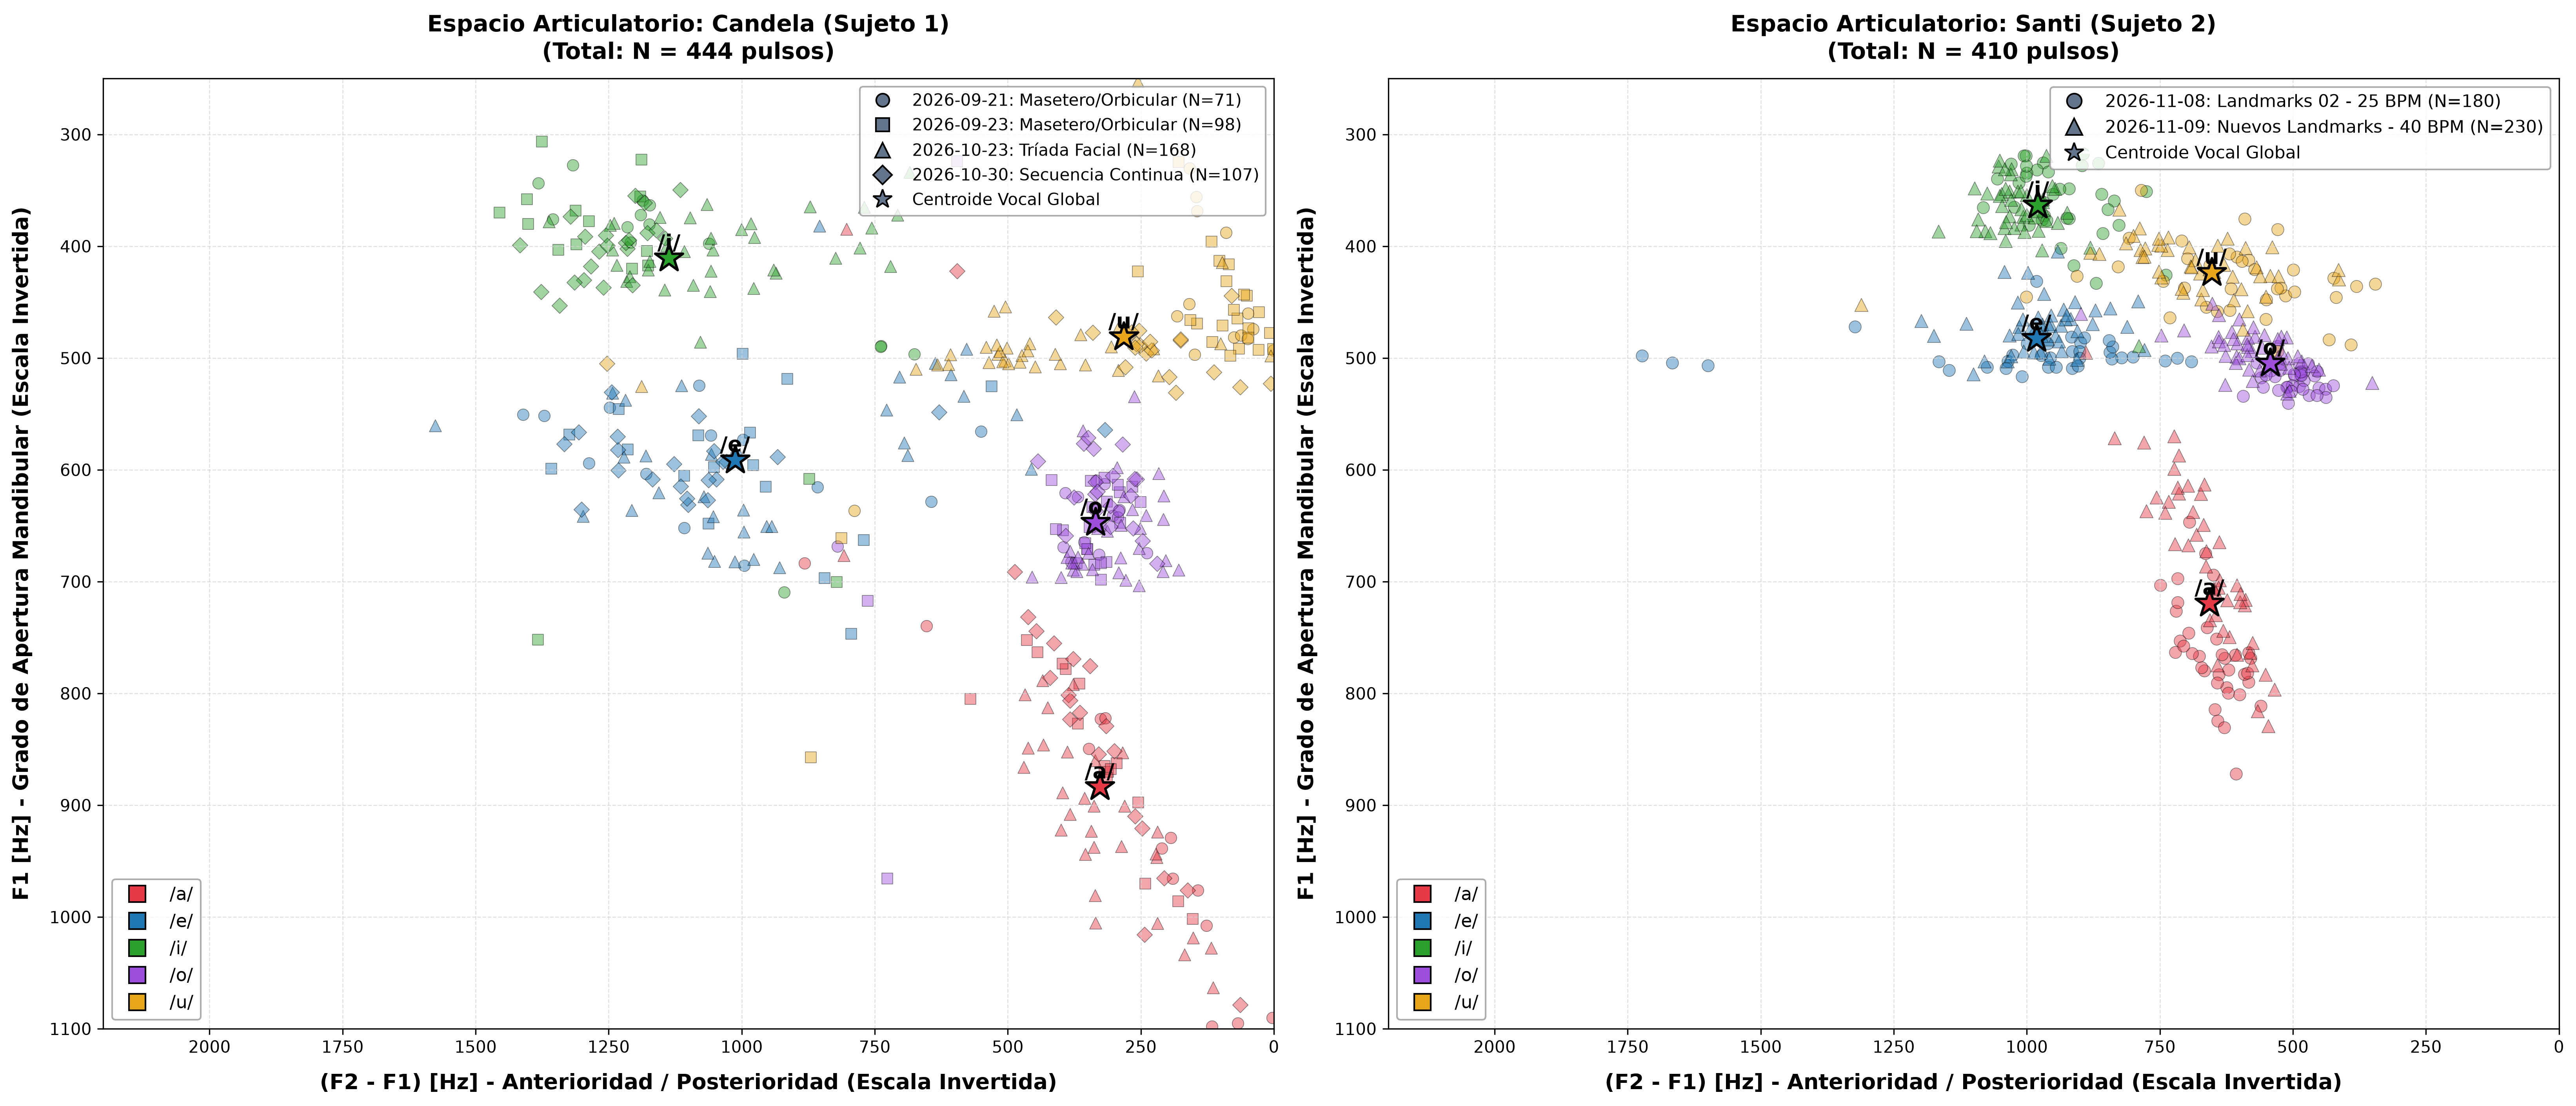
\includegraphics[width=0.98\textwidth]{comparativa_inter_sujeto_lado_a_lado_marcadores_por_sesion.png}
    \caption{Comparativa inter-sujeto lado a lado: Sujeto 1 (Candela, izquierda) vs Sujeto 2 (Santi, derecha) en escalas normalizadas idénticas, con marcadores geométricos específicos por fecha y sesión experimental.}
    \label{fig:comparativa_inter_sujeto_sesiones}
\end{figure}

\subsection{Conclusiones Fisiológicas Inter-Sujeto}
\begin{enumerate}
    \item \textbf{Efecto de Escala de Tracto Vocal:} El Sujeto 1 opera con valores de $F_1$ sistemáticamente superiores a los del Sujeto 2 en todo el repertorio vocálico ($\Delta F_1 \approx 50 - 164\,\text{Hz}$). Esto es consistente con una cavidad faríngea y oral de menor longitud longitudinal total.
    \item \textbf{Amplitud del Trapecio Vocálico:} El Sujeto 1 exhibe un área articulatoria periférica expandida, con $(F_2 - F_1)$ abarcando desde $282\,\text{Hz}$ en /u/ hasta $1137\,\text{Hz}$ en /i/. El Sujeto 2 presenta un espacio mucho más centralizado y compacto.
    \item \textbf{Implicancia para la Decodificación Mioeléctrica:} Estas discrepancias acústicas confirman que un decodificador silente no puede entrenarse sobre targets absolutos en Hertz sin un proceso de calibración o normalización cruzada (como la transformación en bandas críticas de Bark o la alineación geométrica de Procrustes sobre el colector latente).
\end{enumerate}

\end{document}
